% !TeX document-id = {ac384373-0975-4c4e-b6b2-65611dc82067}
% !TeX TXS-program:compile = txs:///pdflatex/[--shell-escape]
\documentclass[a4paper,12pt]{article}

\usepackage[T2A]{fontenc}
\usepackage[russian]{babel}
\usepackage[intlimits,namelimits]{amsmath}
\usepackage{amssymb}
\usepackage{mathtools}

\usepackage{indentfirst}
\usepackage{icomma}
\usepackage{graphicx}
\usepackage{geometry}
\usepackage{setspace}
\usepackage{fancyhdr}
\usepackage{titlesec}

\usepackage{minted}

\usepackage[bibstyle=gost-numeric,citestyle=numeric-comp]{biblatex}

\usepackage{hyperref}

\addbibresource{biblio.bib}

\geometry{a4paper, nomarginpar, left=20mm, right=10mm, top=20mm, bottom=20mm}

\setlocalecaption{russian}{ref}{Список использованной литературы}

\newcommand\Vect[1]{{\boldsymbol{#1}}}
\newcommand{\dd}{\mathrm{d}}
\newcommand{\diag}{\operatorname{diag}}
\renewcommand{\Re}{\operatorname{Re}}
\renewcommand{\Im}{\operatorname{Im}}
\renewcommand{\exp}{\operatorname{e}}
\renewcommand{\imath}{\mathrm{i}}

\newcommand{\mintedlabel}[1]{\phantomsection\label{\detokenize{#1}}}

% \DeclarePairedDelimeter\bra{\langle}{|}
\DeclarePairedDelimiter\ket{|}{\rangle}
\DeclarePairedDelimiter\abs{\lvert}{\rvert}
\DeclarePairedDelimiterX\commut[2]{[}{]}{#1,#2}

\titlespacing{\section}{\parindent}{3.5ex plus 1ex minus .2ex}{2.3ex plus .2ex}

\fancypagestyle{plain}{%
	\fancyhf{}%
	\fancyfoot[R]{\thepage}%
	\renewcommand{\headrulewidth}{0pt}%
	\renewcommand{\footrulewidth}{0pt}%
}

%%%%%%%%%%%%%%%%%%%%%%%%%%%%%%%%%%%%%%%%%%%%%%%%%%%%%%%%%%%%%%%%%%%%%%%%%%%%%%%%

\makeatletter
\def\@sect[#1]#2{%
	\refstepcounter{app@section}
	\setcounter{equation}{0}
	\addcontentsline{toc}{section}{Приложение~\theapp@section}
	{%
		{
			\raggedleft%
			\normalfont%
			Приложение~\theapp@section\par%
		}%
		\Large\bfseries%
		#2%
		\par%
	}
	\vskip 3ex
}
% This is supposed to be "starred" version, but it doesn't have sense in the
% appendix, so we simply repeat above definition.
\def\@ssect#1{%
	\refstepcounter{app@section}
	\addcontentsline{toc}{section}{Приложение~\theapp@section}%
	{%
		{%
			\raggedleft%
			\normalfont%
			Приложение~\theapp@section\par%
		}%
		\Large\bfseries%
		#1%
		\par%
	}%
	\vskip 3ex
}

\renewcommand\appendix{%
	\newpage%
	\newcounter{app@section}
	\setcounter{app@section}{0}
	%\setcounter{equation}{0}%
	\renewcommand\theapp@section{\Asbuk{app@section}}
	\renewcommand\theequation{\theapp@section\arabic{equation}}
	%%% We need to redefine \section command here...
	%%% NB: this is messy, VERY messy (see GOST for autoreferat!)
	\renewcommand{\section}{%
		\secdef\@sect\@ssect
	}
}

%%%%%%%%%%%%%%%%%%%%%%%%%%%%%%%%%%%%%%%%%%%%%%%%%%%%%%%%%%%%%%%%%%%%%%%%%%%%%%%%

\begin{document}
	\onehalfspacing
	\pagestyle{plain}

	\begin{titlepage}
		\begin{center}
			{%
				\scshape
				Министерство высшего образования и науки Российской Федерации\\
			}
			федеральное государственное бюджетное образовательное \\
			учреждение высшего образования \\
			«Иркутский государственный университет»
			(ФГБОУ ВО «ИГУ»)\\
			Физический факультет
		\end{center}
		\vspace*{3em}

		\begin{flushright}
			\begin{minipage}{60mm}
				Кафедра теоретической физики\\
				И.о. зав. кафедрой\\
				Доцент, к.ф.-м.н., \underline{\hspace{20mm}} Ловцов С.В.
			\end{minipage}
		\end{flushright}
		\vspace*{4em}

		\begin{center}
			\large%
			Курсовая работа\\[2ex]\
			\Large\bfseries%
			Оценка качества численного решения уравнения осцилляций нейтрино в среде
		\end{center}

		\vspace*{3em}

		\begin{flushright}
			\begin{minipage}{70mm}
				Работы выполнил: \underline{\hspace{30mm}}
				\\[2ex]
				Руководитель: \underline{\hspace{30mm}}\\[2ex]
				Нормоконтроль: \underline{\hspace{30mm}}
			\end{minipage}
		\end{flushright}

		\vfill
		\begin{center}
			Иркутск 2024
		\end{center}
	\end{titlepage}

	\setcounter{page}{2}

	\thispagestyle{empty}
	\tableofcontents

	\newpage

	\section{Введение}
	Нейтринная физика сейчас является одним из рубежей современной физики. Также благодаря своим необычным свойствам нейтрино являются важным элементом для построения моделей за пределами стандартной модели.

	Нейтрино - это общее название электрически нейтральной фундаментальной частицы

	% \newpage
	\section{Уравнение нейтринных осцилляций в среде}
	Когда активные флэйворные нейтрино распространяются в веществе, на их
	эволюционное уравнение влияют эффективные потенциалы из-за когерентного
	взаимодействия со средой посредством реакций нейтрального и заряженного
	токов. Таким образом, влияние среды можно описать в терминах потенциалов, в
	которых распространяются нейтрино, зависящим от состава среды, электрической
	нейтральности, намагниченности (ориентации спинов), скоростей частиц среды.

	Когда три известных состояния флейвора \(\ket{\nu_{\alpha}}(\alpha= e, \mu, \tau)\) являются линейными комбинациями состояний \(\ket{\nu_{i}}\) c массами \(m_{i}(i=1,2,3)\), состояния флейворных нейтрино являются суперпозицией состояний
	массовых нейтрино
	\begin{equation}\label{eq:11}
		\ket{\nu_{\alpha}}=\sum_{i}U_{\alpha i}^{*}\ket{\nu_{i}},
	\end{equation}
	Коэффициенты \(U_{\alpha i}\) являются элементами унитарной матрицы
	смешивания \(U\), называемой матрицей Понтекорва–Маки–Накагавы–Сакаты\footnote{Pontecorvo–Maki–Nakagawa–Sakata (PMNS)}. Для нейтрино Дирака матрица обычно выражается как
	\begin{equation}
		U=O_{23}\Gamma O_{13}\Gamma^{\dagger}O_{12},
	\end{equation}
	где \(O_{ij}\) ортогональные матрицы, представляющие повороты на углы \(\Theta_{ij}\in[0, \pi/2]\) в соответствующих плоскостях, в то время как \(\Gamma=\diag(1,1,\exp^{\imath\delta})\)---диагональная матрица, где \(\delta\) меняющаяся в пределах \([0, 2\pi]\).

	Рассмотрим нейтрино \(\nu_{\alpha}\) рожденное в момент времени
	\(t_{0}\) в среде. Состояние системы \(\ket{\Psi(t)}\) для момента времени \(t\geq t_{0}\) можно представить в виде
	\begin{equation}
		\ket{\Psi(t)}=\sum_{\beta}\Psi_{\beta}(t)\ket{\nu_{\beta}},
	\end{equation}
	Причем \(\Psi_{\beta}(t_{0})=\delta_{\alpha\beta}\). Вероятность иметь состояние флейвора \(\beta\) в точке в точке \(r=t (\hbar=c=1)\) равна
	\begin{equation}\label{eq:12}
		P_{\alpha\beta}(r)=|\Psi_{\beta}(r)|^{2}.
	\end{equation}
	После того, как нейтрино покидают среду, амплитуды
	эволюционируют в соответствии с уравнением, которое
	управляет вакуумными колебаниями, решение которого
	проще, если записать его в базисе массовых собственных
	состояний. Используя уравнению \eqref{eq:11}, и обозначив амплитуду вероятности нахождения
	\(\ket{\nu_{j}}\) на краю среды, для \(r\geq r_{*}\) через \(A_{j}=\phi_{j}(r_{*})\), мы получаем
	\begin{equation}\label{eq:13}
		\Psi_{\beta}(r)=\sum_{j=1}^{3}U_{\beta j}A_{j}\exp^{-\imath E_{j}L}
	\end{equation}
	где \(E_{j}=\sqrt{|\Vect{p}|^{2}+m_{j}^{2}}\), а \(L=r-r_{*}\) это расстояние
	пройденное нейтрино в вакууме. Теперь в
	уравнении \eqref{eq:12} мы мы используем выражение \eqref{eq:13} и получаем
	\begin{equation}\label{eq:17}
		P_{\alpha\beta}=\sum_{j}|U_{\beta j}|^{2}|A_{j}|^{2}+2\sum_{i>j}\Re[U_{\beta i}U_{\beta j}^{*}A_{i}A_{j}^{*}\exp^{-\imath\Delta_{ij}L}].
	\end{equation}
	Величина \(\Delta_{ij}=\Delta m_{ij}/2E\), для \(E=|\Vect{p}|\), представляет собой  волновое число колебаний, связанное с квадратом разности масс
	\(\Delta m_{ij}^{2}=m_{i}^{2}-m_{j}^{2}\).

	В результате задача вычисления \(P_{\alpha\beta}\) сводится к
	определению величин \(A_{j}\), т.е. нахождению амплитуд
	собственных массовых состояний \(\phi_{j}(r)\) внутри среды, при начальном условии \(\phi_{j}(r_{0})=U_{\alpha j}^{*}\). Для релятивистских нейтрино, распространяющихся в обычной материи, после вычитания глобальной фазы уравнение эволюции для этих амплитуд имеет вид
	\begin{equation}\label{eq:14}
		\imath\frac{\dd\Phi(\xi)}{\dd\xi}=[H_{0}+ v(\xi)U^{\dagger}VU]\Phi(\xi),
	\end{equation}
	где \(\Phi^{T}(r)=(\phi_{1}(\xi),\phi_{2}(\xi),\phi_{3}(\xi))\), \(U\) - матрица
	смешивания, и \(V=\diag(1,0,0)\), \(\xi=\frac{r}{R_{0}}\), где \(R_{0}=6.96\times10^5\) --- солнечный радиус. Первый член в скобках - это матрица Гамильтона, которая управляет эволюцией флейвора в вакууме \(H_{0}\), он имеет вид:
	\begin{equation}
		H_{0}=\frac{a}{E}
		\begin{pmatrix}
			0 & 0 & 0\\
			0 & b & 0\\
			0 & 0 & 1
		\end{pmatrix},
	\end{equation}
	Здесь \(E\) --- числовое значение энергии нейтрино в МэВ, а \(a=4.35196\times10^6\) и \(b=0.030554\) --- безразмерные параметры. Второй член в скобках учитывает эффекты, связанные с когерентным взаимодействием нейтрино с фоновыми частицами. Величина \(v(\xi)\) обозначает разницу между эффективными потенциальными энергиями \(\nu_e\) и \(\nu_{\mu,\tau}\). 

Так как \(O_{12}\) и \(\Gamma\) коммутируют, матрица PMNS мможет быть зписана так: \(U=O_{23}\Gamma O \Gamma^{\dagger}\), где \(O=O_{13}O_{12}\). Также комутаторы \([V,O_{23}], [V,\Gamma], [H_0,\Gamma]\) равны нулю. Следовательно можно получить
	\begin{equation}\label{eq:15}
		\imath\frac{\dd\Psi(\xi)}{\dd\xi}=[H_{0}+ v(\xi)W]\Psi(\xi),
	\end{equation}
	где \(\Psi(\xi)=\Gamma^{\dagger}\Phi(\xi)\), а \(W=O^{\dagger}VO\). То есть
	 \begin{equation*}\label{eq:16}
  		W=
  		\begin{pmatrix}
  		c_{13}^{2}c_{12}^{2} & c_{12}s_{12}c_{13}^{2} & c_{12}c_{13}s_{13}\\
  		c_{12}s_{12}c_{13}^{2} & s_{12}^{2}c_{13}^{2} & s_{12}c_{13}s_{13}\\
  		c_{12}s_{13}c_{13} & s_{12}c_{13}s_{13} & s_{13}^{2}
  		\end{pmatrix},
  	\end{equation*}
	где \(c_{ij}=cos\theta_{ij}\), а \(s_{ij}=sin\theta_{ij}\). Также необходимо задать определенную форму функции \(v(\xi)\). Для Солнца мы используем экспоненциальный профиль электронной плотности
	\begin{equation}
		v(\xi)=\gamma \exp^{-\eta \xi},
	\end{equation}
 	где  \(\gamma=6.5956 \times 10^4\) и \(\eta=10.54\).

	Как правило, осциллирующие интерференционные члены в уравнении \eqref{eq:17} в среднем равны нулю для нейтрино, пролетающих большое расстояние до Земли. При таких обстоятельствах средняя вероятность обнаружения \(\nu_\beta\) в детекторе на Земле определяется некогерентной суперпозицией
	\begin{equation}
		\langle P_{\alpha\beta} \rangle=\sum_{j}|U_{\beta j}|^{2} \rho_{j},
	\end{equation}
	где \(\rho_{j}=|A_{j}|^{2}=|\phi_{j}(r_{*})|^2\) обозначает вероятность того, что нейтрино будет иметь собственное массовое состояние на поверхности звезды. Так как
	\begin{equation}
		\sum_{j}^{3} \rho_i=1,
	\end{equation}
	а \(|\psi_{j}(r_{*})|^2=|\phi_{j}(r_{*})|^2\). Мы получаем
	\begin{equation}\label{eq:18}
		\sum_{j}^{3} |\psi_{j}(r_{*})|^2=1,
	\end{equation}
	% \newpage


	\section{Метод численного интегрирования}

	Большинство задач в физике приводят к дифференциальным уравнениям как первого,
	так и второго порядков, одной или нескольких переменных. В этой связи перед
	нами часто встаёт задача найти решение задачи
	\begin{equation}\label{eq:21}
		\frac{\dd y}{\dd t}=g(t,y),\qquad y(t_0)=y_0
	\end{equation}

	Что касается уравнения второго порядка, то его можно представить как систему
двух уравнений первого порядка.

	Методы решения  можно разделить на точные, приближенно-аналитические и
	численные. В точных методах решение разыскивается через элементарные,
	специальные функции или в виде интегралов от них.
  В приближенно-аналитических методах решение ищется либо как предел
  \(y(t)\) некоторой последовательности функций \(y_k(t)\), причем \(y_k(t)\)
  выражается через элементарные, специальные функции или интегралы от них, либо
  как конечный набор таких последовательностей (например, аппроксимация
  полиномами).
  Численные — это методы приближенного вычисления решения \(y(t)\) на
  интервале \((t_0,T)\). К этим методам относят семейство методов Рунге–Кутта и
  методы геометрического интегрирования.

  Ниже мы детально рассмотрим методы Рунге–Кутта, но суть подхода в том, что
  рассматриваемый интервал разбивают на части \(t_1,t_2,...,t_N\) с постоянным
  шагом
	\begin{equation}\label{eq:22}
		\begin{lgathered}
			t_{n+1}=t_n+h,\\
			n=0, 1, 2, 3, 4,\ldots.
		\end{lgathered}
	\end{equation}
	Здесь множество точек \(t_i\) называется узлами сетки, а \(h\) --- шага сетки.

	\subsection{Методы Рунге--Кутта}

	Рассмотрим дифференциальное уравнение \eqref{eq:21}. Пусть \(t_0\) и \(y_0\) это
	числа, а для \(g(t,y)\) существуют непрерывные частные производные до некоторого
	порядка \(n-1\). В таком случае для решения уравнения \eqref{eq:21} существуют
	непрерывные производные до \(n\)-го порядка, как минимум в окрестности точки
	\(t=t_0\). Следовательно получаем такое разложение по формуле Тейлора
	\begin{equation}\label{eq:23}
		\begin{lgathered}
			y(t)=y_0+(t-t_0)y_0^{(1)}+\frac{(t-t_0)^2}{2!}y_0^{(2)}+\ldots+\frac{(t-t_0)^n}{n!}y_0^{(n)}+o(|t-t_0|^{n+1})\\
			y_0^{(j)}=\frac{\dd^j y(t_0)}{\dd t^j}
		\end{lgathered}
	\end{equation}
	Сначала решение дифференциального уравнения найдём в точке \(t=t_0+h\), где
	\(h>0\) --- это некоторое достаточно малое число.
	Тогда из разложения \eqref{eq:23}, выбросив члены \(o(|t-t_0|^{n+1})\), получаем
	\begin{equation}\label{eq:24}
		y(t_0+h)\cong y_0+hy_0^{(1)}+\frac{h^2}{2!}y_0^{(2)}+\ldots+\frac{h^n}{n!}y_0^{(n)}
	\end{equation}
	Производные из \eqref{eq:24} можно вычислить, однако получаемые формулы получаются слишком громоздкими. Поэтому К. Рунге предложил, а В. Кутта развил, идею вместо решения формулы \eqref{eq:24} решать следующие линейные комбинации
	\begin{equation}\label{eq:25}
		y(t_0+h)= y_0+b_1k_1(h)+b_2k_2(h)+\ldots+b_sk_s(h)
	\end{equation}
	где \(b_i\) --- некоторые постоянные коэфиценты с условием, что \(\sum_{i=1}^{s}b_i=1\). \(k_i(h)\) --- это функции, что вычисляются по следущей формуле
	 \begin{equation}\label{eq:26}
		k_i(h)=hg(\zeta_i,\eta_i),\qquad i=1,2,\ldots,s
	\end{equation}
	здесь \(\zeta_i=t_0+c_ih\), а
	\(\eta_i=y_0+a_{i1}k_1(h)+a_{i2}k_2(h)+\ldots+a_{ii}k_{i-1}(h)\) для
	\(i=1,2,\ldots,s\).
	Так и было задано семейство явных методов Рунге-Кутта. В явных методах Рунге-Кутта значения вычисляются только по предыдущим значениям.

	Явные методы Рунге-Кутта требующие \(s\) вычислений правой части \(g\) на одном шаге интегрирования  (\(s\)-стадийные явные методы Рунге – Кутта), имеют следующий вид:
	\begin{equation}\label{eq:2}
		y_{n+1}=y_n+h\sum_{i=1}^{s}b_ik_i,
	\end{equation}
	где
	\begin{equation}\label{eq:2}
		\begin{lgathered}
			k_1=g(t_n, y_n),\\
			k_2=g(t_n+c_2h, y_n+a_{21}k_1h),\\
			k_3=g(t_n+c_3h, y_n+(a_{31}k_1+a_{32}k_1)),\\
			\vdots\\
			k_s=g(t_n+c_sh, y_n+h\sum_{i=1}^{s-1}a_{si}k_i),\\
		\end{lgathered}
	\end{equation}

	Чтобы выбрать конкретный метод, необходимо задать целое число \(s\) (количество
	стадий) и коэффициенты \(a_{ij}\), \(1 \leqslant j < i \leqslant s\),
	\(b_i\), \(i = 1, 2, \ldots, s\) и \(c_i\), \(i = 2, 3, \ldots, s\).
	Матрица
	\(\big(a_{ij}\big)\)
	называется матрицей Рунге–Кутта, тогда как \(b_i\) и \(c_i\) известны как веса
	и узлы. Эти данные обычно предоставляются в виде таблицы:
	\begin{equation*}
	\renewcommand\arraystretch{1.2}
	\begin{array}
		{c|ccccc}
		0\\
		c_2 &a_{21}\\
		c_3 &a_{31} &a_{32}\\
		\vdots &\vdots & &\ddots\\
		c_s& a_{s1} &a_{s2}& \ldots&a_{s,s-1}\\
		\hline
		& b_1 &b_2 &\ldots &b_{s-1} &b_s
	\end{array}
	\end{equation*}

	Явные методы Рунге–Кутта, как правило, непригодны для решения Жестких уравнений, потому что их область абсолютной устойчивости мала. Для решения этой проблемы и были придуманы неявные методы Рунге–Кутта. В неявных методах Рунге-Кутта значения вычисляются как и по предыдущим, так и по последующим значениям. Неявный метод Рунге–Кутта имеет вид
	\begin{equation}
		y_{n+1}=y_n+h\sum_{i=1}^{s}b_ik_i,
	\end{equation}
	где
	\begin{equation}
		k_i=g(t_n+c_sh, y_n+h\sum_{j=1}^{s}a_{ij}k_j),\qquad i=1,2,...,s.\\
	\end{equation}

	Отличие от явного метода заключается в том, сумма по \(j\) доходит до \(s\),
	когда в явном методе только до \(s-1\). Это также влияет на таблицу
	коэффициентов. В отличии от явного случая она не является строго
	нижнетреугольной. Это дает нам такой её вид
	\begin{equation*}
	\renewcommand\arraystretch{1.2}
	\begin{array}
		{c|ccccc}
		c_1 &a_{11} &a_{12} &\ldots &a_{1s}\\
		c_2 &a_{21} &a_{22}&\ldots&a_{2s}\\
		\vdots &\vdots &\vdots &\ddots &\vdots\\
		c_s& a_{s1} &a_{s2} &\ldots &a_{s,s}\\
		\hline
		& b_1 &b_2 &\ldots &b_{s}
	\end{array}
	\end{equation*}

	Также существуют адаптивные методы Рунге-Кутта. Они преднозначены для оценки локальной ошибки усечения одного шага Рунге-Кутта. Это работает благодоря использованию двух методов. Один с порядком \(p\), второй с \(p-1\). Данные два метода имеют общие промежуточные этапы, иными словами переплетены. Благодоря этому затраты на вычисление оценки ошибки меньше, по сравнению с использованием только метода более высокого порядка

	В адаптивном методе во время вычисления размер шага изменяется таким образом, чтобы оценочная ошибка оставалась меньше заранее заданого порога. Если ошибка слишком большая, то вычисления повторяются с меньшим шагом, а если ошибка намного меньше заданого порога, то размер шага увеличивается для экономии времени.

	Выражение для определения шага меньшего порядка
	\begin{equation}
		y_{n+1}^{*}=y_n+h\sum_{i=1}^{s}b_i^{*}k_i,
	\end{equation}
	где \(k_i\) те же, что и для метода более высокого порядка. В таком случае ошибка
	\begin{equation}
		e_{n+1}=y_{n+1}-y_{n+1}^{*}=h\sum_{i=1}^{s}(b_i-b_i^{*})k_i,
	\end{equation}
	равняется (неуверен) \(O(h^p)\). Таблица для такого метода тоже модифицируется.
	Она расширена добавлением \(b_i^{*}\)
	\begin{equation*}
	\renewcommand\arraystretch{1.2}
	\begin{array}
		{c|ccccc}
		c_1 &a_{11} &a_{12} &\ldots &a_{1s}\\
		c_2 &a_{21} &a_{22}&\ldots&a_{2s}\\
		\vdots &\vdots &\vdots &\ddots &\vdots\\
		c_s& a_{s1} &a_{s2} &\ldots &a_{s,s}\\
		\hline
		& b_1 &b_2 &\ldots &b_{s}\\
		& b_1^{*} &b_2^{*} &\ldots &b_{s}^{*}
	\end{array}
	\end{equation*}

	\subsubsection{Метод RKF45}

	Сейчас в большинстве случаев, когда нужно провести расчёт с хорошей точностью применяют метод RKF45. По параметрам он является методом порядка \(O(h^4)\) с оценкой ошибки порядка  \(O(h^5)\). Этот метод является адаптивным.

	Таблица коэффициентов для него
	 \begin{equation*}
	 \renewcommand\arraystretch{1.2}
	 \begin{array}
	 	{c|ccccccc}
	 	0\\
	 	\frac{1}{4} & \frac{1}{4}\\
	 	\frac{3}{8} &\frac{3}{32} &\frac{9}{32} \\
		\frac{12}{13} &\frac{1932}{2197} &-\frac{7200}{2197} &\frac{7296}{2197} \\
		1 &\frac{439}{216} &-8 &\frac{3680}{513} &-\frac{845}{4104} \\
		\frac{1}{2}&-\frac{8}{27} &2 &-\frac{3544}{2565} &\frac{1859}{4104} &-\frac{11}{40} \\
	 	\hline
	 	& \frac{16}{135} &0 &\frac{6656}{12825} &\frac{2856}{56430} &-\frac{9}{50} &\frac{2}{55}\\
		& \frac{25}{216} &0 &\frac{1408}{2565} &\frac{2197}{4104} &-\frac{1}{5} &0
	 \end{array}
	 \end{equation*}

	\subsubsection{Методы Рунге – Кутта при \(s\) = 4 (Наверно его надо удалить?)}

	Формулы имеют вид
	\begin{equation}
		\begin{lgathered}
			y_{n+1}=y_n+\frac{h}{6}(k_1+2k_2+2k_3+k_4),\\
			t_{n+1}=t_n+h,\\
			n=0, 1, 2, 3, 4, ....,\\
		\end{lgathered}
	\end{equation}
	где:
	\begin{equation}
		\begin{lgathered}
			k_1=g(t_n, y_n),\\
			k_2=g(t_n+\frac{h}{2}, y_n+k_1\frac{h}{2}),\\
			k_3=g(t_n+\frac{h}{2}, y_n+k_2\frac{h}{2}),\\
			k_4=g(t_n+h, y_n+hk_3),\\
		\end{lgathered}
	\end{equation}
	Здесь \(y_{n+1}\) является RK4 приближением \(y(t_{n+1})\), а следующее значение \(y_{n+1}\) определяется текущим значением \(y_n\) плюс средневзвешенное значение четырех приращений, где каждое приращение является произведением размера интервала \(h\) и предполагаемого наклона, заданного функцией \(g\) в правой части дифференциального уравнения (рис.\ref{fig:magnus}).
	\begin{itemize}
		\item \(k_{1}\) - наклон в начале интервала, используя и \(y\)(метод Эйлера )
		\item \(k_{2}\) - наклон в середине интервала, используя \(y\) и \(k_{1}\)
		\item \(k_{3}\) - снова наклон в средней точке, но теперь с использованием \(y\) и \(k_{2}\)
		\item \(k_{4}\) - наклон в конце интервала, используя \(y\) и \(k_{3}\)
	\end{itemize}
	\begin{figure}[htb]
		\centering%
		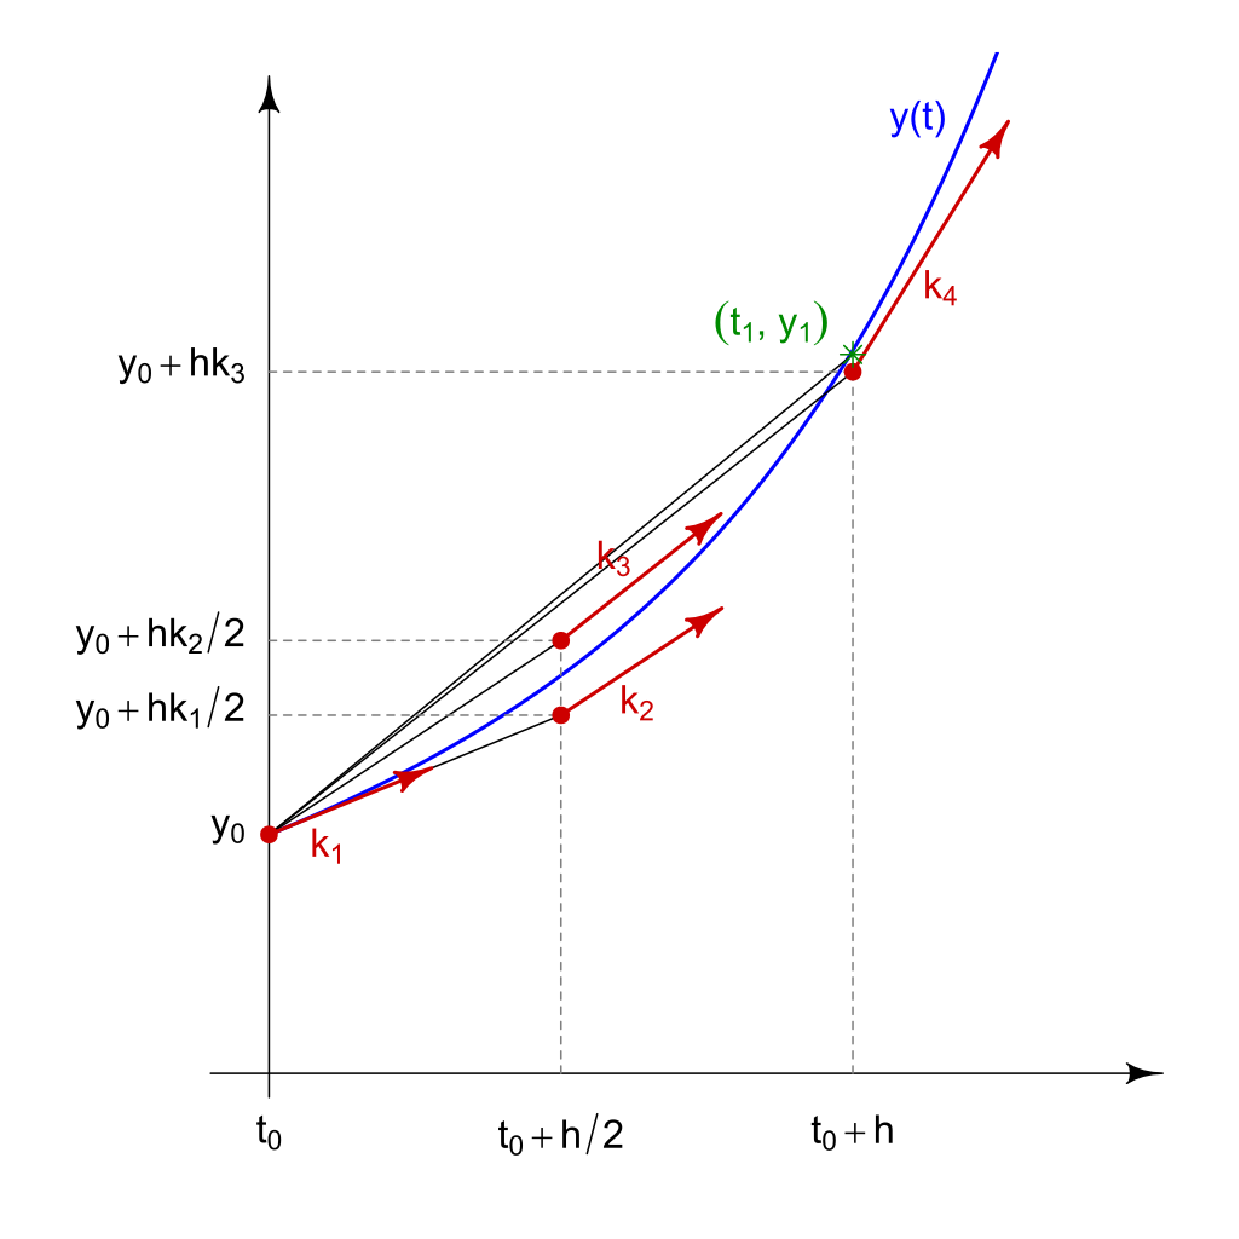
\includegraphics[width=0.8\linewidth]{Ruhgy_koef}
		\caption{\label{fig:magnus}Уклоны, используемые классическим методом Рунге-Кутта}
	\end{figure}

	Метод RK4 является методом четвертого порядка, что означает, что локальная ошибка усечения имеет порядок \(O(h^{5})\), в то время как общая накопленная ошибка составляет порядка\(O(h^{4})\).



	 Метод RK4 попадает в эту структуру. Его таблица
	 \[
	 \renewcommand\arraystretch{1.2}
	 \begin{array}
	 	{c|cccc}
	 	0\\
	 	\frac{1}{2} & \frac{1}{2}\\
	 	\frac{1}{2} &0 &\frac{1}{2} \\
	 	1& 0& 0& 1\\
	 	\hline
	 	& \frac{1}{6} &\frac{1}{3} &\frac{1}{3} &\frac{1}{6}
	 \end{array}
	 \]

	\subsubsection{Метод Дормана – Принца}

	Метод Дормана-Принса состоит из семи этапов, но он использует только шесть оценок функций на шаг, поскольку имеет свойство «Первый такой же, как последний» (FSAL): последний этап оценивается в той же точке, что и первый этап следующего шага. Дорманд и Принс выбрали коэффициенты своего метода так, чтобы минимизировать ошибку решения пятого порядка. В этом главное отличие от метода Фельберга, который построен так, что решение четвертого порядка имеет небольшую погрешность. По этой причине метод Дормана – Принса более подходит, когда для продолжения интегрирования используется решение более высокого порядка, практика, известная как локальная экстраполяция .

	Таблица Бутчера для него
	 \[
	 \renewcommand\arraystretch{1.2}
	 \begin{array}
	 	{c|ccccccc}
	 	0\\
	 	\frac{1}{5} & \frac{1}{5}\\
	 	\frac{3}{10} &\frac{3}{40} &\frac{9}{40} \\
		\frac{4}{5} &\frac{44}{45} &-\frac{56}{15} &\frac{32}{9} \\
		\frac{8}{9} &\frac{19372}{6561} &-\frac{25360}{2187} &\frac{64448}{6561} &-\frac{212}{729} \\
		1&\frac{9017}{3168} &-\frac{355}{33} &\frac{46732}{5247} &\frac{49}{176} &-\frac{5103}{18656} \\
	 	1&\frac{35}{384} &0 &\frac{500}{1113} &\frac{125}{192} &-\frac{2187}{6784}&\frac{11}{84} \\
	 	\hline
		&\frac{35}{384} &0 &\frac{500}{1113} &\frac{125}{192} &-\frac{2187}{6784}&\frac{11}{84}&0 \\
	 	& \frac{5179}{517600} &0 &\frac{7571}{16695} &\frac{393}{640} &-\frac{92097}{339200} &\frac{187}{2100} &\frac{1}{40}
	 \end{array}
	 \]

	\subsubsection{Сравнение методов RK45 и Дормана-Принца}

	
\end{document}

